\documentclass{beamer}
\usepackage{xcolor}
%\usepackage{tikz}
\usepackage{multimedia}


% \usepackage{beamerthemesplit} // Activate for custom appearance

\title{On (mod $n$) Spirals}
\author{Andrew R. Reiter (Veracode, Inc.)\\
Robin Young (UMASS-Amherst)}
\date{\today}

\theoremstyle{mydef}
%\newtheorem{definition}{}
\newtheorem{conj}{Conjecture}[section]
\newtheorem{thm}{Theorem}[section]

\begin{document}

\frame{\titlepage}

%\section[Outline]{}
%\frame{\tableofcontents}

\section{Introduction}
\frame{
\frametitle{Goal of Talk}
A means to teach students how to think mathematically.
\begin{itemize}
\item Show how one can impose definitions to patterns you see.
\item Observations$\rightarrow$Conjecture$\rightarrow$Proof
\item Learn to generalize: dim 2$\rightarrow$dim $d$
\end{itemize}
\begin{center}
\end{center}
Aimed at early high school students, but can be useful to all ages/levels.
}


\frame
{
  \frametitle{Motivation for Play}

  \begin{itemize}
  \item Polar Vortex!\\
  \begin{center}
  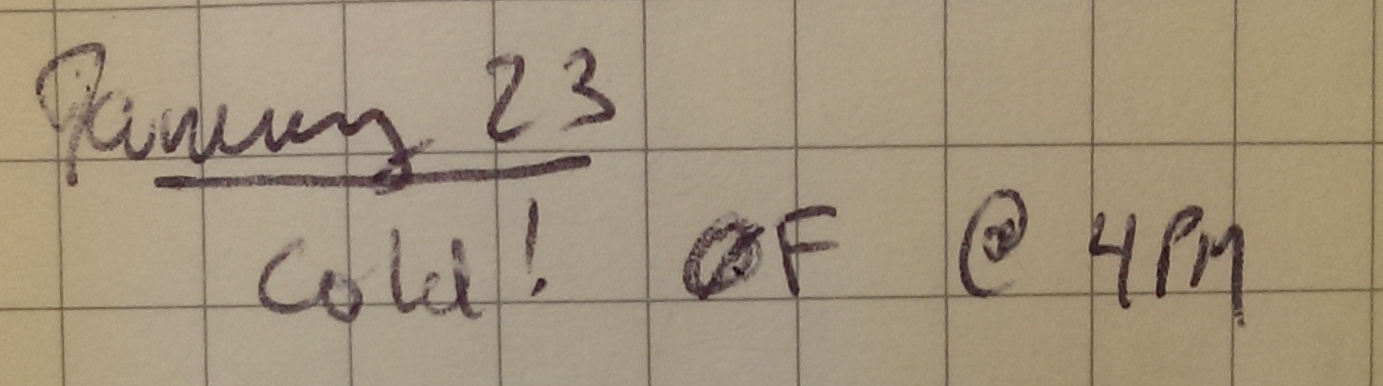
\includegraphics[scale=.15]{images/PolarVortex1.png}
  \end{center}
  \item In bed with flu for a week or so
  \item What to do?\\
  \begin{center}
  MATH!... or at least play with numbers
  \end{center}
  \item Hackathon!
  \end{itemize}  
}



\frame
{
  \frametitle{Orderly Doodling}
 \[
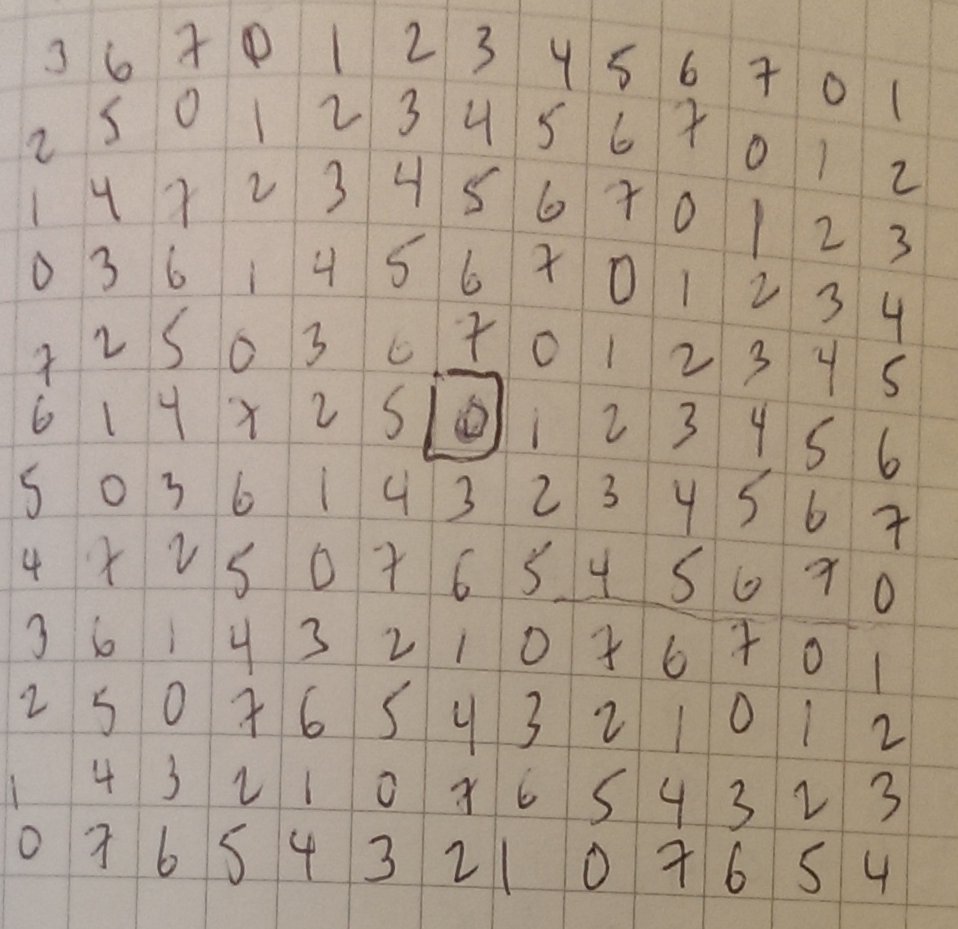
\includegraphics[scale=.15]{images/mod8.png}\quad
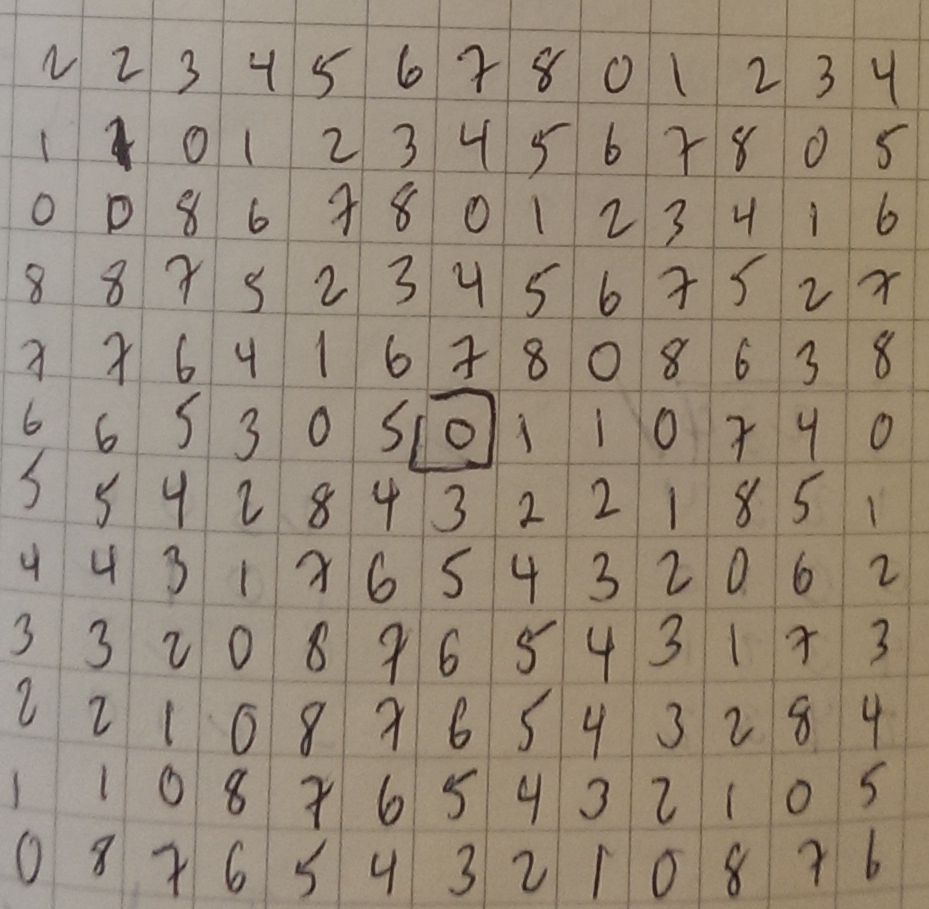
\includegraphics[scale=.15]{images/mod9.png}
\]
}


\frame
{
  \frametitle{What is the process?}
  Select an integer $n \ge 2$, say $n = 3$, noting $\mathbb{Z}_3 = \{ 0, 1, 2\}$
  \begin{center}
  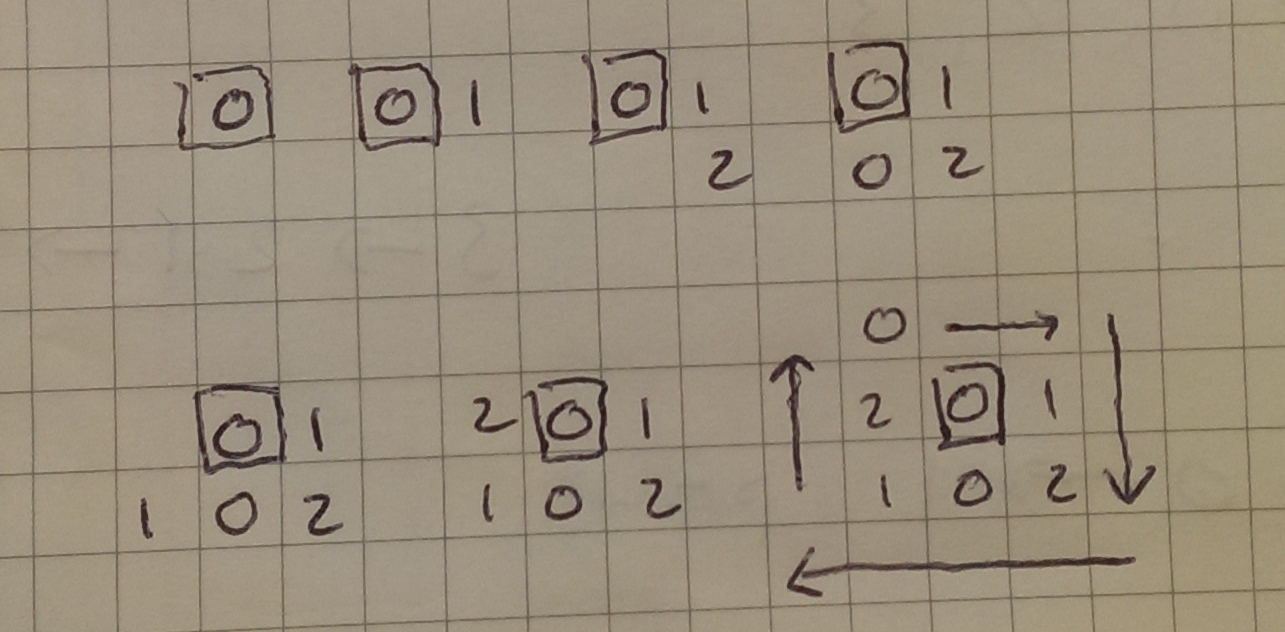
\includegraphics[scale=.1]{images/mod3move.png}
  \end{center}
\tiny
\[  \begin{array}{c}
\boxed{0}
\end{array} 
\rightarrow
%
\begin{array}{cc}
\boxed{0} & 1 \\
\  & \ 
\end{array}
\rightarrow
\begin{array}{cc}
\boxed{0} & 1 \\
\  & 2
\end{array}
\rightarrow
\begin{array}{cc}
\boxed{0} & 1 \\
0 & 2
\end{array}
\rightarrow
\]

\[
\begin{array}{ccc}
\  & \boxed{0} & 1 \\
1 & 0 & 2
\end{array}
\rightarrow
\begin{array}{ccc}
2 & \boxed{0} & 1 \\
1 & 0 & 2
\end{array}
\rightarrow
\begin{array}{ccccc}
\  & 0 & \cdot  & \cdot & \cdot \\
\  & 2 & \boxed{0} & 1 & \cdot \\
\  & 1 & 0 & 2 & \cdot \\
\cdot & \cdot & \cdot & \cdot & \cdot
\end{array}
\]
Formally,
\[
  l_j^* = j-1 \!\!\!\pmod n \quad\text{at site}\quad l_j.
\]

}



\frame
{
  \frametitle{Patterns Seemed Interesting}
\[
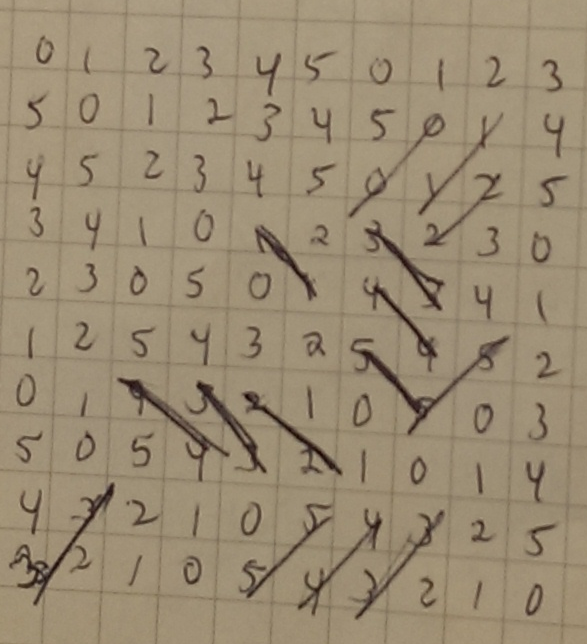
\includegraphics[scale=.2]{images/mod6scratch.png}\quad
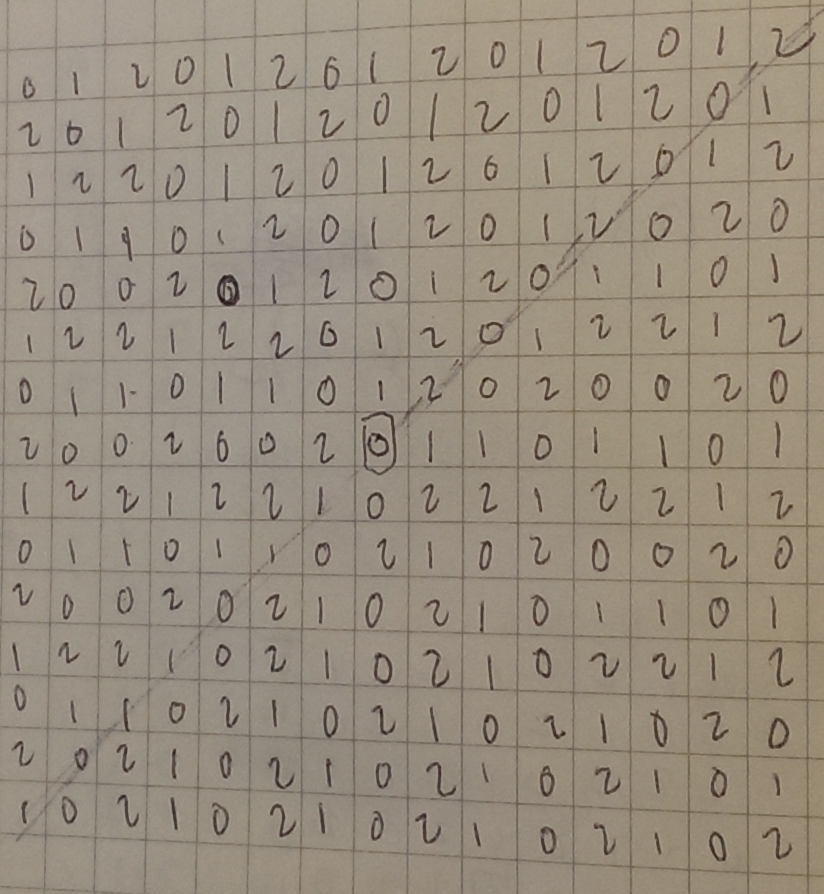
\includegraphics[scale=.15]{images/bigmod3hand.png}
\]

...want larger spirals!
}



\frame
{
  \frametitle{Desire to Automate}

  \begin{columns}
    \begin{column}{.5\textwidth}
     \begin{block}{
     
     \color{black}
  \begin{itemize}
       \color{black}

  \item Want bigger spirals: tedious by hand
  \item Write a program!
    \end{itemize} 
}
% Your text here
    \end{block}
    \end{column}
    \begin{column}{.5\textwidth}
    \begin{block}{}
% Your image included here
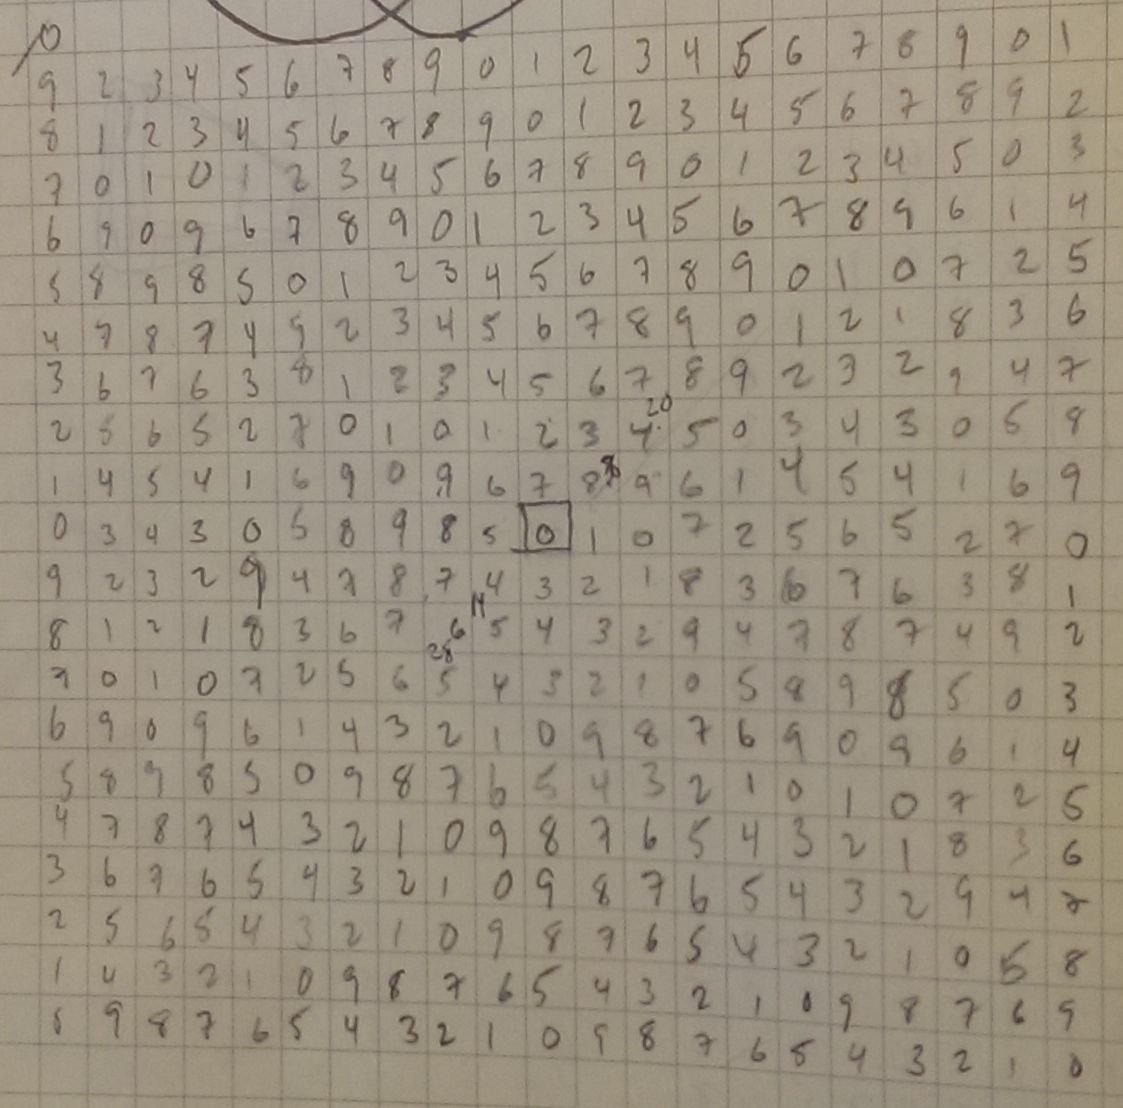
\includegraphics[scale=.15]{images/bigmod10.png}
    \end{block}
    \end{column}
  \end{columns}
  }


\frame
{
\frametitle{Programs Call for Definitions}
\begin{itemize} 
\item \emph{Complete Spiral}
\begin{itemize}
\item Forms a square and
\item Last value assigned is $l^*_i = n-1$
\end{itemize}

\item ``Ond'' is spiral in Swahili
\begin{itemize}
\item First complete spiral achieved is  $Ond^1_n$
\item Subsequent are $Ond^k_n$, $k = 2,3,\dots$.  
\end{itemize}
\item \emph{Iteration Count} is number of times $\mathbb{Z}_n$ used in the $k^{th}$ square
\end{itemize}
}

%% INSERT TIKZ
\frame
{
\begin{center}
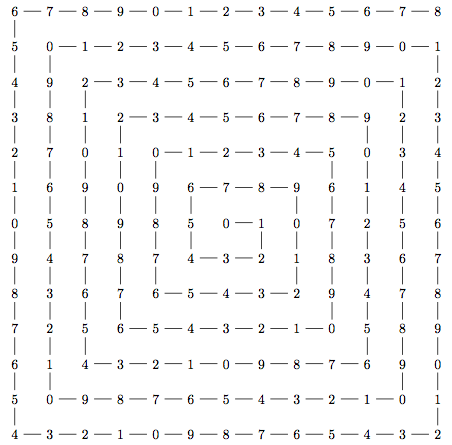
\includegraphics[scale=.5]{images/tikz.png}

Still unwieldy

\end{center}
}

\section{Visuals}
\frame
{
  \frametitle{Visualize the patterns}
  Realize generated $Ond_n^k$ as grayscale graphical images\\
  \vspace{10 mm}
  The map $f : \mathbb{Z}_n \to \mathbb{Z}_{256}$ is defined by a scaled floor function,
\[
   f(j) = \alpha j, \quad \text{where} \quad
   \alpha = \left\lfloor \frac{255}n \right\rfloor
\]
}

\subsection{Square Lattice}
\frame
{
  \frametitle{Square Lattice}

  \[
 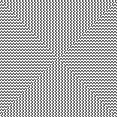
\includegraphics[scale=.8]{images/Ond-N3-k39.png}\quad
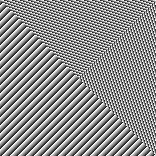
\includegraphics[scale=.5]{images/Ond-N8-k39.png}\quad
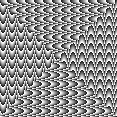
\includegraphics[scale=.5]{images/Ond-N9-k39.png}
\]
  \[
  Ond_3^{39}\quad Ond_{8}^{39}\quad Ond_{9}^{39} \text{ respectively}
  \]
}

\frame
{
\begin{center}

\includegraphics[scale=.24]{images/Ond-N31-k39.png}
\end{center}
}


\frame
{
  \frametitle{Automation to Conjecture}
  
  \begin{itemize}
  \item Initial image creation guessed at size of generated spiral
  \item Is there some formula for \emph{Ond side length} and \emph{iterations}?
  \item Can I use $(n, k, \ldots)$ to determine this?
  \end{itemize}

}

\frame
{
 \frametitle{Generate Data and Observe}
  Output \emph{iteration} and \emph{side length} data when generating \emph{Ond} images
\begin{center}
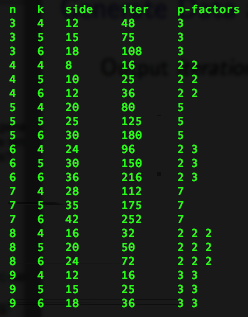
\includegraphics[scale=.5]{images/sometab.png}

\end{center}
\begin{itemize}
\item Included prime factors of $n$ to output to add information
\end{itemize}
}

\frame
{
 \frametitle{Generate Data and Observe}
  Output \emph{iteration} and \emph{side length} data when generating \emph{Ond} images
  
\begin{center}
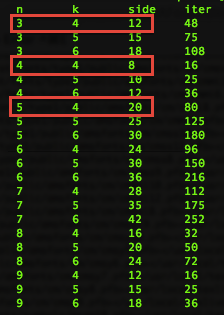
\includegraphics[scale=.5]{images/sometab-box.png}
\end{center}

\begin{itemize}
\item Side lengths:  $Ond_3^{4} > Ond_4^{4} < Ond_5^{4}  \implies$ non-linearity
\end{itemize}
}


\frame
{
  \frametitle{}
  \begin{thm}%[Length of Sides of $Ond^k_n$]
\label{lenthm}
\footnotesize
Let $s$ denote the greatest square divisor of $n$.
The complete spiral $Ond^k_n$ has the following structure:
\begin{enumerate}[(i)]
\item If $\lambda$ is the length of the sides of $Ond^k_n$, then
\begin{equation}
  \lambda = \frac{kn}{\sqrt{s}}.
\label{lambda}
\end{equation}
\item If $\xi$ is the iteration count of $Ond^k_n$, then
\begin{equation}
  \xi = \frac{k^2n}{s}.  
\label{xi}
\end{equation}
\end{enumerate}
\end{thm}
}

\frame
{
  \frametitle{Greatest Perfect Square Divisor of $n$}
  
  Write down $Ond_n^1$, determine side length, solve $\lambda = \frac{n}{\sqrt{s}}$ for $s$.
}

\frame
{

\begin{proof}[Proof of the Conjecture]
\begin{itemize}
  \item $n\ge 2$ is fixed
  \item $\lambda$  complete spiral side length, $\xi$ iteration count
  \item Spiral is square $\implies \xi n = \lambda^2 \implies n \vert \lambda^2$.
  \item $p \vert n$ with $p$ prime $\implies p \vert \lambda^2 \implies p \vert \lambda$
  \item $s$ is greatest square divisor of $n \implies n = q^2_1 q_2$
  \begin{itemize}
  \item $q_2$ is square-free
  \item $s = q_1^2$.
  \end{itemize}
   
  \item  $n \vert \lambda^2 \implies q_1^2\vert\lambda^2 \implies q_1|\lambda$ and $\implies q_2 \vert (\frac{\lambda}{q_1})^2$
  
  \item $q_2$ is square-free $\implies q_2\vert (\frac{\lambda}{q_1})$ and $\lambda = k q_1 q_2$ for $k\in \mathbb{Z}_{+}$.  
  \item $n\vert\lambda^2$ for any such $\lambda$, thus $\lambda = k q_1 q_2$ is the side of the $k$-th complete spiral $Ond^k_n$.

  \item $\lambda = \frac{kn}{\sqrt{s}}$ follows since $\sqrt{s} = q_1$
  \item $\xi = \frac{k^2n}{s}$ follows since $\xi = \frac{\lambda^2}{n}$.  
  \end{itemize}
\end{proof}
}

\frame
{
\frametitle{Generalize!}

  \begin{itemize}
  \item Generalize in dimension: increase $d$
  \item Generalize in shape
  \item Think of geometrically: filling an area
  \begin{itemize}
  \item more abstractly looking at when $n \vert f(d)$
  \end{itemize}
  \end{itemize}
}

\frame
{
 \frametitle{Generalize in Dimension}
  \begin{itemize}
  \item Generalize to $d$-dim hypercube by looking at $n \vert \lambda^d$
  \begin{itemize}
  \item Difficult to visualize
      \end{itemize}
   \end{itemize}
  \begin{thm}
Let $n\vert \lambda^d$ for $d=2, 3, \ldots$. Let $n = qm^d$ where $m \in \mathbb{N}$ and $q$ is $d$-power 
free. Let $q$ be defined in terms of it's prime factors, $p_j$, as
\[
	q = \prod\limits_{j=1}^{r} p_j^{e_j}\quad \text{with}\ \text{each}\quad e_j < d.
\]
then
\[
	\lambda = k m \prod p_j \quad k = 1, 2, 3, \ldots
\]
\end{thm}
\begin{itemize}
\item Note that $m^d$ is the greatest $d$-power divisor of $n$
\item Proof is similar to $d=2$ proof.
\end{itemize}
}


\frame
{
  \frametitle{Other Shapes: Centered Hexagons}
  \begin{itemize}
  \item Centered hexagonal numbers are $CH_d = 3d(d+1)+1$
  \item Investigate $n \vert CH_d$
  \item Not all $n$ will satisfy!
  \begin{itemize}
  \item $n=2, \ldots, 6$ don't work but $n = 7, 13, 19, 31, 37, \ldots$ will
  \end{itemize}
  \end{itemize}
\[
  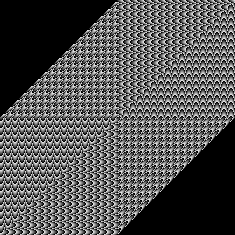
\includegraphics[scale=.45]{images/hex-sp-N7-k34.png}\quad
  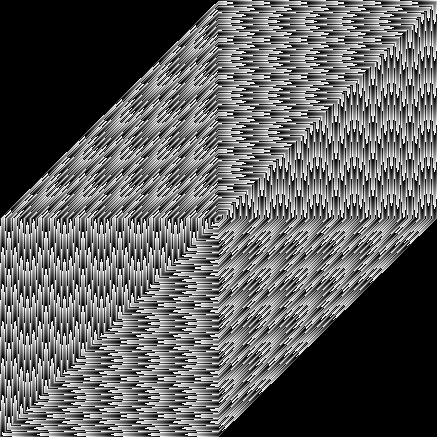
\includegraphics[scale=.25]{images/hex-sp-N37-k12.png}
\]
\[
 HexOnd_{7}^{34}\text{ and }HexOnd_{37}^{12}
 \]
}

\frame
{
\begin{center}
  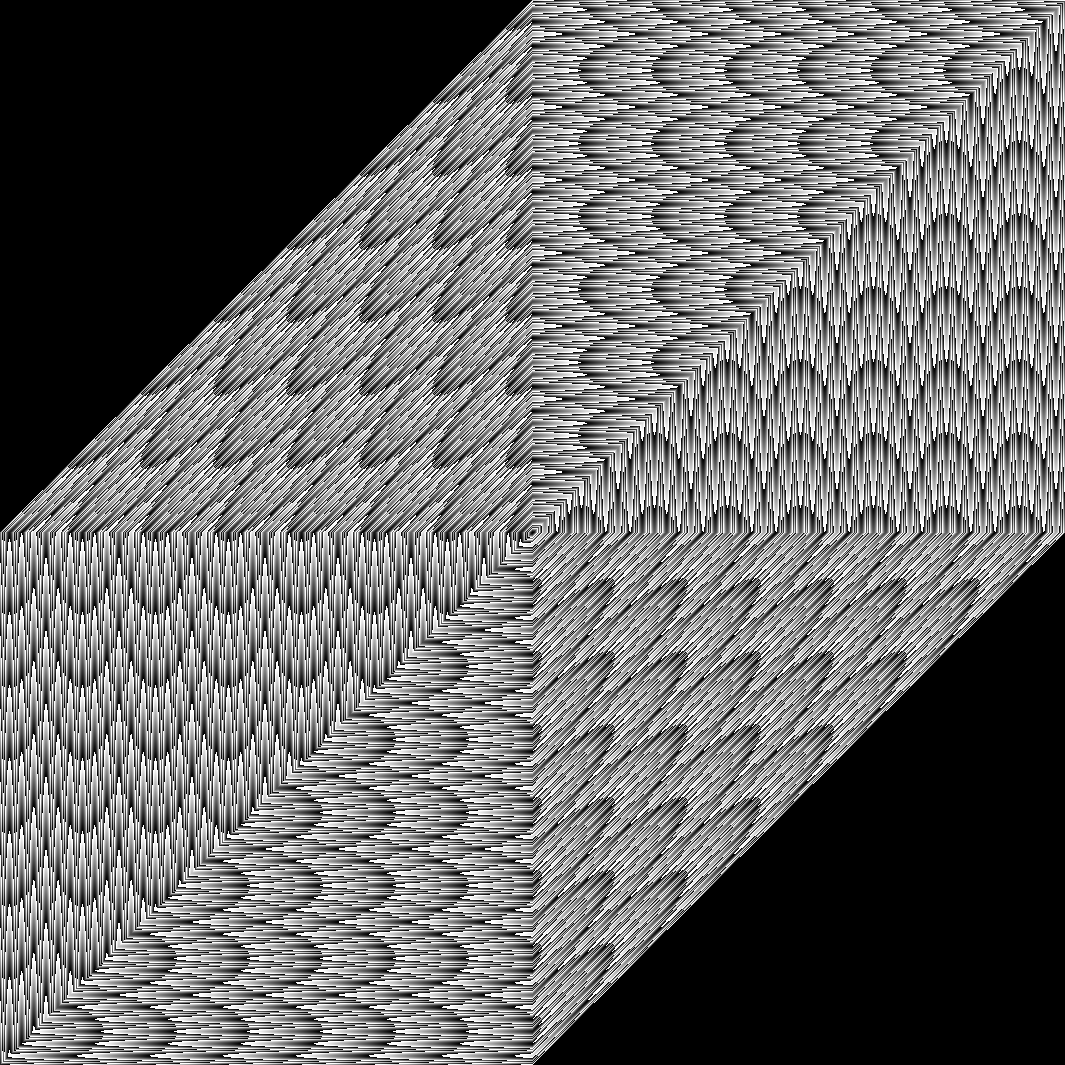
\includegraphics[scale=.24]{images/hex-sp-N73-k15.png}  
 \end{center}
  }
  
\frame
{
  \frametitle{Other Shapes: Triangles}
  \begin{itemize}
  \item Triangle numbers are $T_d = \frac{d(d+1)}{2}$
    \item Investigate $n \vert T_d$
 \end{itemize}
 \begin{center}
 \[
  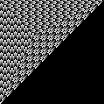
\includegraphics[scale=.75]{images/tri-sp-N7-k29.png}\quad
  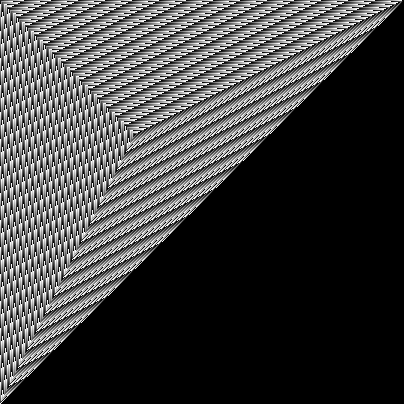
\includegraphics[scale=.25]{images/tri-sp-N27-k29.png}
\]
\[
 TriOnd_{7}^{29}\text{ and }TriOnd_{27}^{29}
 \]
 \end{center}
}

\frame
{
\begin{center}
\[
 TriOnd_{36}^{29}\text{ and }TriOnd_{39}^{29}
 \]
\[
  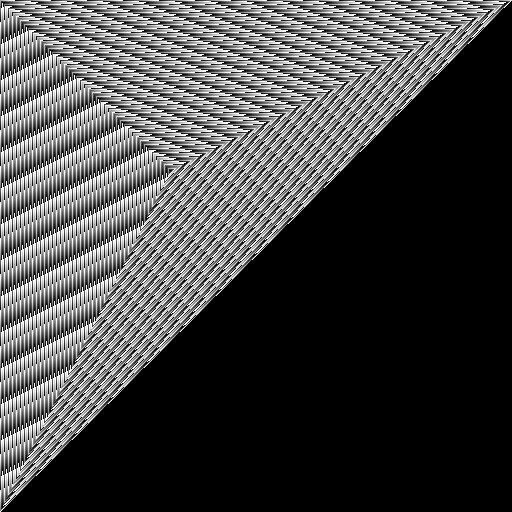
\includegraphics[scale=.25]{images/tri-sp-N36-k29.png} \quad
  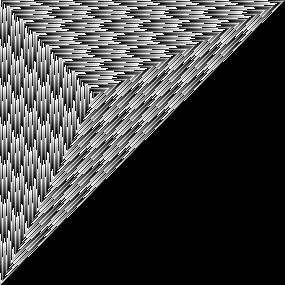
\includegraphics[scale=.45]{images/tri-sp-N39-k29.png}
  \]
Note the bias by using right triangle
 \end{center}
}

\section{Conclusion}
\frame{
\frametitle{So what is all this?}
\begin{itemize}
\item Show how one can impose definitions to patterns you see.
\item Observations$\rightarrow$Conjecture$\rightarrow$Proof
\item Learn to generalize
\end{itemize}
\begin{center}
A means to teach how to think mathematically!
\end{center}
}
\frame
{
  \frametitle{Things to Explore}
  \begin{itemize}
  \item Other 2 dimensional lattice shapes
  \item Non-hypercube shapes in $>2$ dimensions
  \item Addition of $Ond$
  \item Random $Ond$: Select $n_0$ from some distribution, cycle through $\mathbb{Z}_{n_0}$ once, choose $n_1$,  cycle through $\mathbb{Z}_{n_1}$, ...
  \end{itemize}
}
\frame
{
  \frametitle{Thank You!}
  We invite you to please take a paper if you are interested in this topic. For code and visualizations, please go to:
  
  \begin{center}
  https://github.com/cwcomplex/modNspirals
  \end{center}
  \begin{itemize}
  \item Robin Young of UMASS-Amherst
  \item Veracode, Inc -- Hackathon!
  \item Jared Carlson of Veracode
  \end{itemize}
  Contact: areiter@veracode.com, young@math.umass.edu
}
\end{document}
